\documentclass[a4paper]{article}

\usepackage[utf8]{inputenc}
\usepackage{mlmodern}
\usepackage[T1]{fontenc}
\usepackage{textcomp}
\usepackage[dutch]{babel}
\usepackage{amsmath, amssymb,physics}
\usepackage{tcolorbox}
\pagestyle{fancy}
\usepackage{fancyhdr}
\usepackage{preamble}
\usepackage{hyperref}
\usepackage{transparent}
\newcommand{\incfig}[1]{%
    \def\svgwidth{\columnwidth}
    \import{./figures/}{#1.pdf_tex}
}
\pdfsuppresswarningpagegroup=1
\title{PH2202: Thermal Physics}
\begin{document}
% \maketitle
    \begin{titlepage}

\newcommand{\HRule}{\rule{\linewidth}{0.5mm}} % Defines a new command for the horizontal lines, change thickness here

\center % Center everything on the page
 
%----------------------------------------------------------------------------------------
%	HEADING SECTIONS
%----------------------------------------------------------------------------------------

\textsc{\LARGE IISERK}\\[1.5cm] % Name of your university/college
% \textsc{\Large  }\\[0.5cm] % Major heading such as course name
% \textsc{\large Minor Heading}\\[0.5cm] % Minor heading such as course title

%----------------------------------------------------------------------------------------
%	TITLE SECTION
%----------------------------------------------------------------------------------------

\HRule \\[0.4cm]
{ \huge \bfseries Probability 1}\\[0.4cm] % Title of your document
\HRule \\[1.5cm]
 
%----------------------------------------------------------------------------------------
%	AUTHOR SECTION
%----------------------------------------------------------------------------------------

\begin{minipage}{0.4\textwidth}
\begin{flushleft} \large
\emph{Author:}\\
Sabarno \textsc{Saha} % Your name
\end{flushleft}
\end{minipage}
~
\begin{minipage}{0.4\textwidth}
\begin{flushright} \large
\emph{Instructor:} \\
Dr. Soumya \textsc{Bhattacharya} % Supervisor's Name
\end{flushright}
\end{minipage}\\[2cm]

% If you don't want a supervisor, uncomment the two lines below and remove the section above
%\Large \emph{Author:}\\
%John \textsc{Smith}\\[3cm] % Your name

%----------------------------------------------------------------------------------------
%	DATE SECTION
%----------------------------------------------------------------------------------------

{\large \today}\\[2cm] % Date, change the \today to a set date if you want to be precise

%----------------------------------------------------------------------------------------
%	LOGO SECTION
%----------------------------------------------------------------------------------------

% \includegraphics{logo.png}\\[1cm] % Include a department/university logo - this will require the graphicx package
 
%----------------------------------------------------------------------------------------

\vfill % Fill the rest of the page with whitespace

\end{titlepage}



    \newpage
    \tableofcontents
    \newpage 
        \section{Introduction} 
    The course introduces us to the fundamentals of thermal physics and will end with statistical physics. The instructor for this course is Dr. Koushik Datta. 
    The recommended reading for this course is "Heat and Thermodynamics" by Zemansky and Dittman. 
    \subsection{Readings} 
    \begin{itemize}
        \item \emph{An Introduction to Thermal Physics } by D.V. Schroeder
        \item \emph{Thermodynamics} by Enrico Fermi
    \end{itemize}
    
    
    \section{Internal energy of Ideal Gas}
    We use some elementary equations already taught in CH1201. We will be using the ideal gas 
    equation and the $1^{st}$ Law of Thermodynamics. 
    \begin{align*}
        PV &= NRT \\ 
        dU &= TdS - pdV + \mu dN
    \end{align*}
    We assume the fact that the internal energy of the system, something we will define later,
    depends on the variables entropy(S), volume(V) and no of moles(N). The first term of equation
    2 above change in heat energy $dQ = TdS$ and work done on the system $dW = -PdV$ and 
    chemical potential $\mu dN$. 
    \begin{align}
        dU &= \pdv{U}{S}dS - \pdv{U}{V}dV + \pdv{U}{N}dN \\ 
        % \tag{Comparing this to the first law} 
        T &= \pdv{U}{S}dS\\ 
        P &= - \pdv{U}{V}dV \\ 
        \mu &= \pdv{U}{N}dN 
    \end{align}
    The chemical potential is a new term added in this course. %definition to added here:
    So chemical potential essentially refers to the change in internal energy on adding or 
    subtracting a molecule. Essentially when we add an infinitesimally small number of molecules
    say dN, we have the chemical potential term to be $\mu dN$.%\\[5]
    
    \begin{problem}
      We need to find a closed form expression of the internal energy of an ideal gas in terms 
      of its state variables
    \end{problem}

    \\[5]
    \emph{Answer: } We introduce one more equation into solving for the closed form expression i.e. the 
    equipartition of energy.
    \begin{align}
        U &= \frac{3}{2} NRT \nonumber\\ 
        \Rightarrow T & = \frac{2U}{3NR} 
    \end{align}
    From here its just algebra to find the solution to the problem
    \begin{align}
        \pdv{U}{S} = T = \frac{2U}{3NR}\nonumber\\ 
        % \tag{Integrating the equation gives us.}
        \Rightarrow \ln (U) = \frac{2S}{3NR}+ f(V,N) 
    \end{align}
    So we now need to obtain the function \(f\). For this again we will use a different 
    thermodynamic equality namely the ideal Gas equation.
    \begin{align*}
        & PV = NRT\\
        \Rightarrow & P = \frac{NRT}{V}\\ 
        \tag{Using (3)}
        & \pdv{U}{V} = -P = \frac{NRT}{V} = -\frac{2U}{3V} \\ 
        \tag{Differentiating (6)}
        & \pdv{(\ln U)}{V} = \pdv{f}{V} \\ 
        &\Rightarrow \frac{1}{U}\pdv{U}{V} = \pdv{f}{V}\\ 
        \tag{Substituting the deriavtive}
        &\Rightarrow \frac{1}{U} \qty(-\frac{2U}{3V}) = \pdv{f}{V} \\ 
        & \Rightarrow \partial{f} = -\frac{2}{3} \frac{\partial{V}}{V} \\ 
        \tag{Integrating}
        & \Rightarrow f = -\frac{2}{3} \ln(V) + \ln(g(N))
    \end{align*} 
    Other than the fucntion g(N) we have found the closed form expression of internal energy of 
    ideal gas which is
    \begin{align}
        &\ln U = \frac{2S}{3NR} - \frac{2}{3} \ln(V) + \ln(g(N)) \nonumber\\ 
        \Rightarrow & U = g(N)V^{-2/3}\exp\qty(\frac{2S}{3NR})  
    \end{align}
    Now to figure out the value of g(N), we need to apply a property of the variables we are working
    with. Now given a thermodynamic variable, it can either be intensive or extensive in nature.
    Intensive variables or properties are such properties that do not depend on the amount of substance
    we are measuring the variable of. For example, the melting point of a liquid is an intensive property
    i.e. if we add more liquid, the melting point still remains the same. In contrast there are 
    extensive properties or variable which depend on the amount of the substance taken. For example,
    mass is a very trivial example of an extensive property. \\ 
    So all the properties that we are dealing with here are extensive. I will try to give a motivation 
    of why they are extensive, but the fact that a property is extensive or intensive is a purely 
    experimental result. \\ 

    We first talk about entropy, which is a concept that measures the disorder in a system. Suppose
    you have a system A and then a system B , the disorder of the combined system will depend on the 
    combined A and B, meaning it is not an inherent property of the substance we are taking. Same goes 
    the case for volume. I mean if we add two systems with different volumes, their resultant volume 
    will be the combined volume. The no of moles(N) is also an extensive property, since it is just a 
    scaled analogy to mass. \\ 
    Similary if we talk about the equipartition of energy, then the internal energy is directly dependent
    on the no of moles, which makes it an extensive property. \\ 

    Thus we will scale the system now where 
    \(S\mapsto \lambda S, V \mapsto \lambda V \quad \text{and} \quad N\mapsto \lambda N \) where 
   \(\lambda\) is some scaling factor. As a result \(U\mapsto \lambda U\). Keeping this in mind we 
   perform the aforementioned mapping on equation (7).
   \begin{align*}
       U' &= g(\lambda N)(\lambda V)^{-2/3}\exp\qty(\frac{2 \lambda S}{3 \lambda NR}) \\ 
          & = g(\lambda N) \lambda^{-2/3} V^{-2/3}\exp\qty(\frac{2S}{3NR}) \\ 
          & = g(\lambda N) \lambda^{-2/3} \frac{U}{g(N)} \\ 
       \Rightarrow \lambda U &=  g(\lambda N) \lambda^{-2/3} \\ 
       \Rightarrow g(\lambda n) &= \lambda^{5/3}g(N)
   \end{align*}
   This is a fairly easy function equation to solve we just set N=1 and \(\lambda = N\). 
   \begin{align}
       \tag{where k is some constant}
       g(N) = kN^{5/3}
   \end{align}
   Now plugging this equation in (7), We get our final closed form solution of the problem we want.\\
   \begin{center}
       \large
       \fbox{ 
       \begin{equation*}
           U = kN^{5/3} V^{-2/3}\exp\qty(\frac{2S}{3NR})  
       \end{equation*}
       }
   \end{center}
   {\hfill \blacksquare}


       \section{The Zeroth Law}
   In any study of something, we have to choose what properties to study or not 
   study for our causes. The importance of context has a large role to play. We concern ourself 
   with an effective description of the \emph{system}(defined later) we are studying. 
   For example, in fluid dynamics we do not need to concern ourself with the individual motions 
   of each particle of the fluid. Studying that to understand fluids would be unecessarily cumbersome.
   Instead, what we do is that we take averages of certain properties over a certain volume to 
   reduce the small epsilon changes that takes place in each configuration of the molecules. 
   Here we discuss that a bit further.

   \subsection{Macroscopic and Microscopic points of view}
   \subsubsection{Macroscopic POV}
   Let's get the definition of the macroscopic POV straight of the way. Zemansky and Dittman refer
   to the macroscopic description of the system as a \emph{few fundamental measureable} properties of 
   the system we are trying to study.   

   So we can elaborate this further. In order to get an effective description of our system for the 
   cases of thermodynamics,
   we do not need to consider very small changes in the microscopic description of the system. 
   We need to select a lengthscale and a timescale for our measurements. So what we do is we only 
   consider changes that happen within our length-scale i.e. if we have a length-scale of 1-10 
   metres, we should not consider changes that requires something like a vernier calliper to 
   measure. Essentially, if we do not see that small changes in a length scale smaller than this
    affect our effective description, we should not take into account that when we consider the 
   macroscopic definition of the system. Similarly we also choose a timescale and ignore anything 
   that happens outside of our timescale. The choice of length and time scales are heavily dependent 
   on the context of the study we are doing. After doing so, we move on to an important stage.

   Now we have to choose some variables that both effectively describe our system effectively and 
   can be measured by us. The point of choosing length and time scales will much more evident now.
    The choice of macroscopic variables should be such that they do not evolve within that length 
   or time scale. Qualita-tively we are effectively choosing variables such that our system is 
   somewhat static over that length and time scale. Going the other way, we can also check when our
    system is static and then check for constant quantities. 
   \subsubsection{Microscopic POV}
   ZD defines a microscopic description to be a description involving the internal structure of a 
   system and then based on those assumptions calculating system wide characteristics. This will 
   be discussed later, inevitably when we talk about Statistical mechanics later.
   \subsubsection{Conclusion}
   Whatever description we give be it Macroscopic or microscopic, they must eventually give the 
   same result because they are essentially the same thing. The emergence macroscopic variables 
   of a system is just an averaging of some microscopic variables. For example, Pressure is just 
   averaging out the linear momenta of particles over some length and time scales.
   \subsection{Definitions}
   \begin{itemize}
       \item \emph{System: } The part of the universe we are studying.
       \item \emph{Surroundings: }The part of universe which is not the system.
       \item \emph{Boundary: }The seperating between the system and the surroundings.
       \item \emph{Open System: }A system where exchange of matter and energy is allowed between the system and the surroudings.
       \item \emph{Closed System: }A system where exhange of energy is allowed but exchange of matter is not.
       \item \emph{Isolated System: }A system where exchange of both energy and matter are not allowed.
       \item (not a definition) We can exchange energy two ways, by heating the system and by doing mechanical work of the system.
       \item \emph{Adiabatic Wall: }A boundary that allows no exchange of heat energy to take place.
       \item \emph{Diathermic Wall: }A boundary that allows heat transfer, but no transfer of matter is allowed.
       \item \emph{State of a system: }When we talk about a system, we talk about its macroscopic variables. The state of the system is the state of these variables.
       \item \emph{Mechanical Equilibrium: }When the resultant force and torque on a system are 0, i.e. \(\sum_{i=1}^{n}F_i + \sum_{i=1}^{k}\tau_i = 0\)
       \item \emph{Chemical Equilibrium: }When the system exhibits bo change in composition.
       \item \emph{Thermal Equilibrium: }This will be defined much better later. For now, it is just when heat exchange stops between systems.
       \item \emph{Thermodynamic Equilibrium: }If the system is in all of the equilibria above, then it is thermodynamic equilibrium.
   \end{itemize}
   \begin{tcolorbox}[colback=blue!5!white,colframe=blue!75!black,arc=0mm,title=Note]
     For all systems we talk about here, unless otherwise mentioned, are implicitly assumed to be in thermodynamic equilibrium.
   \end{tcolorbox}
   There is a very good reason for this assumption. In thermodynamics, we always deal with macroscopic 
   quantities, i.e. microscopic quantities that are coarse grained. Now, if we do not have the system in 
   thermal equilibrium, we will not have an effective description of the system using macroscopic 
   quantities. The microscopic quantities might vary enormously, causing the macroscopic definition to 
   not be as effective of a description as we would like.
   \subsection{Thermal Equilibrium and Temperature}
   We now talk about the concept of thermal equilibrium and temperature. 
   \begin{tcolorbox}[colback=blue!5!white,colframe=blue!75!black,arc=0mm,title=Theorem]
       Let us have a system defined 
       by macroscopic quantities \(x,y,z\). We claim that there will exist a function \(f(x,y,z) = 0\), called the \textbf{Equation of state}.
   \end{tcolorbox}
   We will try to give a motivation for why this is true. The proper foundations of this theorem lie 
   in Gibbs' paper on heterogenous systems, with something called Gibbs' phase rule. However, that might be a problem here, 
   as the phase rule uses the concept of temperature, whereas we have not defined what temperature is. So we will use the same inherent 
   concept used in Gibbs' phase rule, i.e. the fact that the system is in thermodynamic equilibrium.

   Let us define a coordinate space where the $x_i^{th}$ coordinate is the $i^{th}$ macroscopic variable. Here, we have three macroscopic variables, 
   namely, $x,y,z$. Suppose, we have an equilibrium point. What we mean by an equilibrium point is that the, 
   the system will undergo minimal change under minimal change of $x,y,z$. Now, around equilibrium points, we have seen 
   that macroscopic variables are well defined, i.e. macroscopic variables effectively describe the system. Thus, at any particular time, given 
   the values of the three macroscopic quantities, it represents a unique point in the coordinate space. Thus, we have, around 
   some neighbourhood of the equilibrium points, we can define a function \(F\) such \(F(x,y,z)\) represents a 
   unique point in coordinate space. Now  we are just left to show that \(F(x,y,z) = c\) for some constant c. We have to show that it 
   is equal to a constant, otherwise the function \(f\) stated in the theorem will also depend on other variables, other 
   than the given macroscopic variables. Now by definition of thermodynamic equilibrium, the system will not undergo a large amount 
   of change with respect to time. And it will depend only on the macroscopic coordinates as it these coordinates 
   effectively describe a system. Now we assume that \(F(x,y,z)\) is continuous and differentiable, otherwise, 
   the system might drastically change with a small change in x,y and z. Since, at equilibria we define that there is minimal change,
   \begin{align*} 
       &\pdv{F}{x}dx  =0 \\ 
       &\pdv{F}{y}dy = 0 \\ 
       &\pdv{F}{z}dz = 0 \\ 
       \Rightarrow & dF = \pdv{F}{x}dx+\pdv{F}{y}dy+\pdv{F}{z}dz = 0 \\ 
       \tag{where c is a constant}
       \Rightarrow & F = c 
   \end{align*}
   We define \(f(x,y,z) = F(x,y,z)-c = 0\). Thus we provide the motivation for the theorem above.
   **\textbf{This section is still under review}**
   \subsubsection{Thermal Equilibrium}
   We define two systems A and B such that they are seperated by a diathermic wall, and the whole composite system 
   A+B is isolated from the surrounding by an adiabatic wall.
   \begin{center}       
       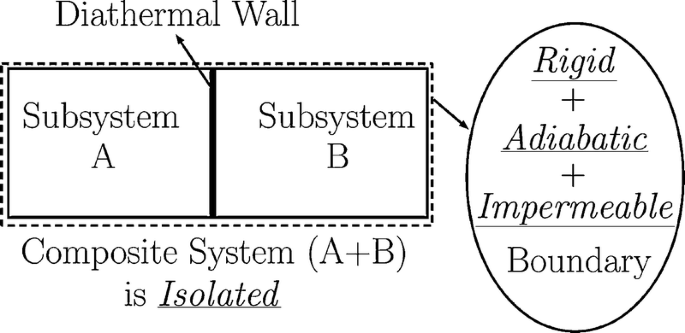
\includegraphics[width =3.0in]{thermequilibria.png}
   \end{center}
   We let subsystem A and subsystem B interact with each other for an indefinite period of time, we define that thermal equilibrium will be reached.
   \begin{tcolorbox}[colback=blue!5!white,colframe=blue!75!black,arc = 0mm,title=Definition]
     Thermal equilibrium is the state acheived by Two or more systems characterized by a restricted set of parameters having been 
     seperated by a diathermic wall.
   \end{tcolorbox}
   We have defined that for a system in thermodynamic equilibrium, there exists an equation of state, for both subsystem A and subsystem B. 
   This leads us to the Zeroth law of thermodynamics
   \subsubsection{The Zeroth Law}
   
   \begin{tcolorbox}[colback=blue!5!white,colframe=blue!75!black,arc = 0mm,title=Definition]
   If A and B are individually in thermal equilibrium with C. Then A and B are in thermal equilibrium with each other.
   \end{tcolorbox}

   The zeroth law suggests that there might exist some physical quantity that is the SAME for systems in thermal equilibrium with each other. 
   We call the physical quantity temperature. We can then redefine the concept of thermal equilibrium, as if the temperature of two systems are the same, then they are in thermal equilibrium. 
   


   
   \section{The First Law}
   lol
   \subsection{Mathematical digression}
   \subsection{Quastistatic Process}
   \subsection{Some Common Thermodynamic Processes}
   \subsection{Adiabatic Lapse Rate}


   
\end{document}

